\documentclass[12pt]{article}
\usepackage[fleqn]{amsmath}
\usepackage[document]{ragged2e}
\usepackage{amsfonts}
\usepackage{amssymb}
\usepackage{setspace}
\usepackage{textcomp}
\doublespacing
\usepackage{amsthm}
\theoremstyle{definition}
\newtheorem{definition}{Definition}[section]
\usepackage{graphicx}
\graphicspath{ {plots/} }
\usepackage[margin=3cm]{geometry}
\usepackage{caption}
\usepackage{subcaption}
\usepackage[section]{placeins}
\usepackage{float}
\usepackage[numbers,sort&compress]{natbib}

\begin{document}
\begin{titlepage}
    \begin{center}
        
        \LARGE
        \textbf{Parameter Estimation for Infinite L\'{e}vy Processes via Sequential Monte Carlo}

        
        \vspace{1.5cm}
        
\includegraphics[scale=1.2]{university}\\
        \vspace{1.5cm}
        
        \large
        \textbf{Liew Kuang Chen Joel A0004624U}

        \large
        \textbf{Department of Mathematics} \\
		\textbf{Supervisor: Professor Zhou Chao}\\
        
        \vfill
        \small
        An honours thesis submitted in partial fulfillment for the degree of\\
		Bachelor of Science (Honours) in Quantitative Finance
        

        
        

        
    \end{center}
\end{titlepage}


\section*{Acknowledgements}
\justify
First, I would like to express my deepest appreciation to Professor Zhou Chao for his patient teaching and the time and effort that he took from his busy schedule to meet me for bi-weekly meetings. Thank you for the positive feedback and the encouragement throughout this period. \\
\\
Second, I would also like to thank Associate Professor Ajay Jasra for taking time off to meet me even though I am not his FYP student. The great passion and knowledge that he possesses in the field of Sequential Monte Carlo had inspired me to strive for excellence in this FYP. Thank you for your patience and guidance.\\
\\
Third, I want to give a special mention to my coursemates: Samuel, Nige, Shih Chen and Sylvanus. I enjoy the times spent discussing everything under the Sun. You guys have been my pillar of strength for the past 4 years.\\
\\
Fourth, I would like to show appreciation to my family and my girlfriend, Li Ling. They have been very supportive and understanding throughout my University Life, without which I will not be who I am today.\\
\\
Last, I would like to thank God for the many inspirations that He had given me during this ardous project journey. He has been my emotional fortitude and source of strength when things were not working out well in life. Thank you for bringing people into my life who had shaped me to become who I am today.\\
\newpage
\section*{Abstract}
Unforseen events can jolt Financial Markets and cause prices to `jump'. As a result, our pricing models should be able to capture such characteristics or we risk mispricing financial instruments. For this paper, we will first introduce the concept of L\'evy process. Next, the paper will familiarise the reader with the concept of Sequential Monte Carlo. Lastly, we will use this new simulation method to retrieve the posterior estimates and attempt to create a profitable trading strategy with the estimates.
\newpage

\tableofcontents
\newpage

\section{Introduction}
\subsection{Background}
We live in a very uncertain World - Financial Crises, acts of Terrorism, uncertain Central Bank Policies, Geopolitical risks etc, all of which could result in spikes of volatility, and therefore jumps in Markets. As a result, the traditional idea of modelling log-prices using Brownian Motion does not fully capture the characteristics of prices in the Financial Markets. Hence, one can perhaps model these prices using the L\'{e}vy Process. In fact, it has been established by that the L\'{e}vy Process is an attractive alternative to Affine Jump Diffusion Models (Brownian motion and Compound Poisson process) \cite{carr2004time}.
Within the family of the L\'{e}vy Process, there are 2 main branches - Finite Activity Models and Infinite Activity Models. The work of Li, Wells and Yu (2006) shows that the Infinite Activity Models can approximate the AJDs and is more robust in capturing the dynamism of the daily returns of the S\&P500 \cite{li2008bayesian}.
\subsection{Project Scope}
This paper firstly gives an introduction of the L\'{e}vy Process and Infinite Activity Models. Next, it acquaints one with the Sequential Monte Carlo Sampler by methodically building upon the concepts of Perfect Monte Carlo and Importance Sampling to derive the Sequential Importance Sampling and then the Sequential Monte Carlo Sampler. Next, this paper seeks to replicate the work of Jasra, Stephens, Doucet and Tsagaris (2011) - using the SMC Algorithm to retrieve the posterior parameters of interest. Lastly, this paper proposes a possible trading strategy to generate returns. In short my contributions for this project are:
\begin{itemize}
\item Combined and simplified the work of Li (2006) and Jasra (2011)
\begin{itemize}
\item simplified the posterior distribution from Li (2006) by introducing a result from Jasra (2011)
\item the resulting posterior distribution has 1 lesser dimension to simulate from
\item introduced the SMC Algorithm from Jasra (2011), instead of the MCMC from Li (2006), which has greatly cut down the time to get the estimate of the parameters.
\item tested the SMC Algorithm to check if the posterior estimates lie within the 95\% credible interval
\end{itemize}
\item Proposed Trading Strategy
\begin{itemize}
\item introduced a novel approach of using posterior parameters to generate returns from the instrument
\item provided a clear and logical framework for refining trading strategies
\item explored the use of simple moving average and exponential moving average with the posterior parameters to create trading systems
\item experimented on the use of multiple trading strategies to create a portfolio of trading strategies that seeks to outperform the traditional buy and hold
\end{itemize}
\end{itemize}
\newpage

\section{Preliminaries}

\subsection{The L\'{e}vy Process}
In this paper, we will be using the Variance Gamma model from the family of Infinite Activity L\'{e}vy Processes. For the uninitiated, we will first go through the basics.
\theoremstyle{definition}
\begin{definition}{L\'{e}vy Process}\\
A L\'{e}vy Process, $X_{t}$, is a cadlag stochastic process on $(\Omega,\mathcal{F}_{t},P)$,with $X_{0}=0$ and has the following properties:\\
1. Independent increments: $X_{t+j+1} - X_{t+j} \perp X_{t+k+1} - X_{t+k}, \forall k,j \ge 0 , k \neq j$\\
2. Stationary increments: The Law of $X_{t+h} - X_{t}$ does not change for any $t$.\\
3. Stochastic continuity: For any $\epsilon>0, \lim_{h\rightarrow 0} P(|X_{t+h}-X_{t}|>\epsilon) = 0$
\end{definition}
\justify The L\'{e}vy Process also satisfies the Infinite Divisibility property.
\begin{definition}{Infinite Divisibility} \\
For $n\ge 2$, a probability distribution F is infinitely divisibile if there exists $n$ i.i.d. random variables $Y_{1},Y_{2},...$ such that $\sum_{i=1}^{n} Y_{i}$ has distribution F.
\end{definition}
\justify One common distribution satisfying the infinite divisibility condition is the Normal Distribution. If $X \sim N(\mu,\sigma^{2})$, then $X = \sum_{i=1}^{n} Y_{i}$,where $Y_{i} \sim N(\frac{\mu}{n},\frac{\sigma^{2}}{n})$.

\justify Due to fact that L\'{e}vy Processes are semimartingales and that their increments are independent, the process is Markovian and therefore in line with the Efficient Market Hypothesis. Hence, such processes are suitable to model asset prices \citep{li2008bayesian}. 
\subsubsection{Infinite Activity Processes - Variance Gamma}
The probability densities of most L\'{e}vy processes are not known in closed forms. However, their characteristics function $\phi_{X_{t}}(u)$ is as follows:
\begin{center}
$
\phi_{X_{t}}(u) = E[\exp^{iuX_{t}}] = \exp^{-t\psi_{x}(u)},t\ge 0
$
\end{center}


\justify where $\psi_{x}(u)$ is the characteristic exponent of $X$ and satisfies the following L\'{e}vy-Khintchine formula \citep{cont2004financial}
\begin{center}
$\psi_{x}\equiv -i\mu u + \frac{\sigma^{2}u^{2}}{2} + \int_{R_{0}} (1-\exp^{iux}+iux1_{|x|<1})\pi (dx) $\\
where $R_{0} = R$ \textbackslash $\{0\}$ and $\pi$ is a $R_{0}$ Radon measure and \\
$\int_{R_{0}} |x|^{2} \pi (dx)< \infty \qquad \int_{R_{0}} \pi (dx) < \infty$
\end{center}

Unlike the Finite Activity models (such as the Merton Jump Model) under the family of L\'{e}vy Processes, the infinite-activity models allow infinite jumps within a finite time interval. Hence,
\begin{center}
$\int_{R_{0}} \pi (dx) \not< \infty$
\end{center}

Within the category of Infinite Activity L\'{e}vy Processes, the jump process can have either finite or infinite variation. In the case of the finite/infinite variation, the sum of the absolute distance is finite/infinite over any finite time interval. For this paper, we will only be focusing on the Variance Gamma Process - a member from the Infinite Activity with Finite Variation. This process, $Z_{t}$, is created using a Brownian Motion, $B_{t}$, with drift $\gamma$ and variance $\sigma_{j}^2$, subordinated by an independent gamma process, $G_{t}$, with parameter $\alpha$.
\begin{center}
$dZ_{t} = \gamma dG_{t} + \sigma_{j}\sqrt{dG_{t}}dB_{t}$\\
$G_{t+t_{0}} - G_{t} \sim Ga(\frac{t}{\alpha},\frac{1}{\alpha})$
\end{center}
with the L\'{e}vy measure given by
\begin{center}
$\pi(dx) = \frac{A^{2}_{\pm}\exp(-\frac{A_{\pm}}{B_{\pm}}|x|)}{B_{\pm}|x|}(dx)$
\end{center}
where $A_{\pm}=\frac{1}{v}\sqrt{\frac{\gamma^{2}v^{2}}{4}+\frac{\sigma^{2}}{2} \pm \frac{\gamma v}{2}},B_{\pm}=A^{2}_{\pm}v$. In the case where $\gamma=0$, the jumps are symmetric about 0 \citep{li2008bayesian}.
\begin{figure}[h]
\centering
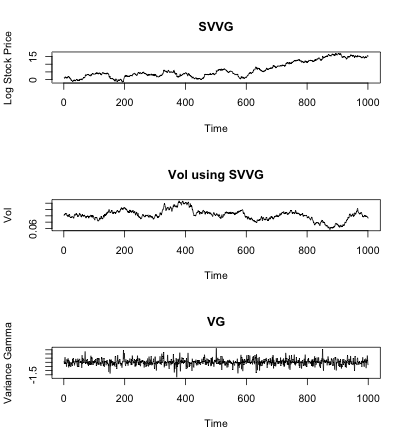
\includegraphics[scale=0.8]{simsvvg}
\caption{A Simulation of the Heston Model with Variance Gamma Process}
\end{figure}
As one can observe in the figure below, the Variance Gamma Process consists of many small jumps with occasional large jumps.
\subsection{Sequential Monte Carlo}
\subsubsection{Perfect Monte Carlo}
Suppose we are able to simulate $N$ i.i.d. random samples/particles $\{\theta_{0:t}^{i},i=1,2,...,N\}$ from a particular distribution (which in this paper, we are refering to the posterior distribution) - $p(\theta_{0:t}|y_{0:t})$. Then, the empirical estimate of this distribution is
\begin{equation}
	\begin{aligned}
		P_{N}(d\theta_{0:t}|y_{0:t}) = \frac{1}{N}\sum_{i=1}^{N}\delta_{\theta_{0:t}^{i}}(d\theta_{0:t})
	\end{aligned}
\end{equation}
where $\delta_{\theta_{0:t}^{i}}(d\theta_{0:t})$ refers to the delta-dirac mass located at $\theta_{0:t}^{i}$. One can then obtain the estimate of $E[f(\theta_{0:t})]$ via
\begin{equation}
	\begin{aligned}
		E[f(\theta_{0:t})]_{est} = \int f(\theta_{0:t}^{i}) \,P_{N}(d\theta_{0:t}|y_{0:t}) = \frac{1}{N}\sum_{i=1}^{N}f(\theta_{0:t}^{i})
	\end{aligned}
\end{equation}
If the posterior variance of $f(\theta_{0:t})$ satisfies \(\sigma^{2} :=\) $E[f(\theta_{0:t})^{2}] - E[f(\theta_{0:t})]^{2} < + \infty $, 
\begin{equation}\label{eq:1}
	\begin{aligned}
		var(E[f(\theta_{0:t})]_{est}) = \frac{\sigma^{2}}{N}
	\end{aligned}
\end{equation}
and by the Strong Law of Large Numbers,
\begin{equation}\label{eq:2}
	\begin{aligned}
		E[f(\theta_{0:t})]_{est} \mathrel{\mathop{\rightarrow}^{\mathrm{a.s.}}_{N \rightarrow \infty}} E[f(\theta_{0:t})]
	\end{aligned}
\end{equation}
Also, if $\sigma^{2} < +\infty$, the Central Limit Theorem holds
\begin{equation}\label{eq:3}
	\begin{aligned}
		\sqrt{N}(E[f(\theta_{0:t})]_{est} - E[f(\theta_{0:t})]) \mathrel{\mathop{\Longrightarrow}_{N \rightarrow \infty}} N(0,\sigma^{2})]
	\end{aligned}
\end{equation}
Unfortunately, it often is difficult to sample from the posterior distribution, especially in high dimensional cases. Markov Chain Monte Carlo (MCMC) methods is a possible alternative, but are unsuited for recursive problems \citep{doucet2001introduction}. Hence, we will introduce a new method in this paper.
\newpage
\subsubsection{Importance Sampling}
One classical method is the use of Importance Sampling method \citep{geweke1989bayesian}. Suppose we are interested in evaluating $E[f(\theta_{0:t})]$. Using a proposal density $\pi(\theta_{0:t}|y_{0:t})$, from which we can easily sample from, we get the following:
\begin{equation}
	\begin{aligned}
		E[f(\theta_{0:t})]_{est} &= \int f(\theta_{0:t}^{i}) \,P_{N}(d\theta_{0:t}|y_{0:t}) \\
		&= \int f(\theta_{0:t}^{i})p(\theta_{0:t}|y_{0:t}) \,d\theta_{0:t} \\
		&= \int f(\theta_{0:t}^{i})\frac{p(\theta_{0:t}|y_{0:t})}{\pi(\theta_{0:t}|y_{0:t})}\pi(\theta_{0:t}|y_{0:t})\,d\theta_{0:t} \\
		&= \int f(\theta_{0:t}^{i})w(\theta_{0:t}^{i})\pi(\theta_{0:t}|y_{0:t})\,d\theta_{0:t} \\
	\end{aligned}
\end{equation}
Since we can easily simulate from $N$ i.i.d. from $\pi(\theta_{0:t}|y_{0:t})$, we can get an estimate of $E[f(\theta_{0:t})]$
\begin{equation}
	\begin{aligned}
		\hat{E}[f(\theta_{0:t})]_{est} &= \int f(\theta_{0:t}^{i})\,\hat{P}(d\theta_{0:t}) \\
		&=\frac{\frac{1}{N}\sum_{i=1}^{N}f(\theta_{0:t}^{i})w(\theta_{0:t}^{i})}{\frac{1}{N}\sum_{i=1}^{N}w(\theta_{0:t}^{i})} \\
		&= \sum_{i=1}^{N}f(\theta_{0:t}^{i})W(\theta_{0:t}^{i}) \\
	\end{aligned}
\end{equation}
where $w(\theta_{0:t}^{i})$ and $W(\theta_{0:t}^{i})$ is known as the importance weights and normalised weights respectively. Note that we are now operating under the new measure 
\begin{equation}
	\begin{aligned}
		\hat{P}(\theta_{0:t}|y_{0:t}) = \frac{1}{N}\sum_{i=1}^{N}\delta_{\theta_{0:t}^{i}}(d\theta_{0:t})W(\theta_{0:t}^{i})
	\end{aligned}
\end{equation}
The Importance Sampling method does not work well in this form (especially in high dimensional cases) \citep{smith2013sequential}. In addition, under $\mathcal{F}_{t+1}$, one has to recompute the weights/normalised weights despite having the weights/normalised weights at $\mathcal{F}_{t}$ - the recursive problem has yet to be solved! However, this has spawned new innovations, one which we will discuss and use in this paper.
\subsubsection{Sequential Importance Sampling (SIS)}
The Importance Sampling Method can be improved to include new information, $\mathcal{F}_{t+1}$, without recomputing $\{\theta_{0:t}^{i},i=1,2,...,N\}$. Using the following fact,
\begin{equation}\label{eq:4}
	\begin{aligned}
		P(A_{n},..,A_{1}|B) = P(A_{n}|A_{n-1},..,B)P(A_{n-1}|A_{n-2},..,B)..P(A_{1}|B)
	\end{aligned}
\end{equation}
we get,
\begin{equation} \label{eq:5}
	\begin{aligned}
		\pi(\theta_{0:t+1}|y_{1:t+1}) = \pi(\theta_{t+1}|\theta_{0:t},y_{1:t+1})\pi(\theta_{0:t}|y_{1:t})
	\end{aligned}
\end{equation}
After iterating,
\begin{equation}
	\begin{aligned}
		\pi(\theta_{0:t+1}|y_{1:t+1}) = \pi(\theta_{0})\prod_{i=1}^{t+1}\pi(\theta_{i}|\theta_{0:i-1},y_{1:i})
	\end{aligned}
\end{equation}
Our weights can then be recursively updated using the following
\begin{equation}
	\begin{aligned}
		W(\theta_{0:t+1}^{i}) \propto W(\theta_{0:t}^{i}) \frac{p(y_{t+1}|\theta_{t+1}^{i})p(\theta_{t+1}^{i}|\theta_{t}^{i})}{\pi(\theta_{t+1}^{i}|\theta_{0:t}^{i},y_{1:t+1})}
	\end{aligned}
\end{equation}
One important case (which we will use) is when we adopt the prior distribution as the importance distribution at $t=0$. However, one drawback of using the SIS method is that one is unable to get the Importance distribution $\pi_{t}(\theta_{1:t})$
\begin{equation}
	\begin{aligned}
		\pi_{t}(\theta_{1:t}) = \int \pi_{1}(\theta_{1})\prod_{k=2}^{t}K_{k}(\theta_{k-1},\theta_{k}) \,d\theta_{1:t-1}
	\end{aligned}
\end{equation}
where $K_{k}(\theta_{k-1},\theta_{k})$ is known as the Markov Kernel. Although there are some approximations used for local random-walk moves, the complexity of the algorithm is $O(N^2)$ and one cannot compute $K_{t}(\theta_{t-1},\theta_{t})$ pointwise \citep{del2006sequential}.
\subsubsection{Sequential Monte Carlo Samplers (SMC)}
The main idea of the Sequential Monte Carlo Samplers is to propose an auxiliary variable technique and introduce artificial backward Markov Kernels, $L_{t-1}$ \citep{del2006sequential}. Given
\begin{center}
$\widetilde{p_{t}}(\theta_{1:t}) = \frac{\widetilde{\gamma_{t}}(\theta_{1:t})}{C_{t}}$\\
$\widetilde{\gamma_{t}}(\theta_{1:t}) = \gamma_{t}(\theta_{t})\prod_{k=1}^{t-1} L_{k}(\theta_{k+1},\theta_{k})$
\end{center}
where $C_{t}$ is the normalisation constant for the unnormalised probability density $\widetilde{\gamma_{t}}(\theta_{1:t})$ and $\gamma_{t}(\theta_{t})$ is the actual unnormalised probability density function of the distribution in question. Suppose, at $\mathcal{F}_{t}$, we have $\{W^{i}_{t},\theta_{0:t}^{i},i=1,2,...,N\}$ approximating $\widetilde{p_{t}}(\theta_{1:t})$
\begin{center}
$\widetilde{p_{t}^{N}}(d\theta_{1:t})=\sum_{i=1}^{N} W^{i}_{t} \delta_{\theta_{1:t}}(d\theta_{1:t})$\\
$W^{i}_{t}(\theta^{i}_{1:t}) = \frac{w^{i}_{t}(\theta^{i}_{1:t})}{\sum_{i=1}^{N} w^{i}_{t}(\theta^{i}_{1:t})}$
\end{center}
where $w_{t}^{i}(\theta_{1:t}^{i})$ is the standard Importance weights. Now, at $\mathcal{F}_{t+1}$, we bring the particles forwards via the Markov Kernel $K_{t+1}(\theta_{t},\theta_{t+1})$. The unnormalised weights is computed using
\begin{equation}
w^{i}_{t+1}(\theta_{1:t+1}) = \frac{\gamma_{t+1}(\theta_{1:t+1})}{\pi_{t+1}(\theta_{1:t+1})} = w^{i}_{t}(\theta_{1:t})\widetilde{w}^{i}_{t+1}(\theta_{t},\theta_{t+1})
\end{equation}
where the incremental weight, $\widetilde{w}^{i}_{t+1}(\theta_{t},\theta_{t+1})$ equals to
\begin{equation}\label{eq:6}
\widetilde{w}^{i}_{t+1}(\theta_{t},\theta_{t+1}) = \frac{\gamma_{t+1}(\theta_{t+1})L_{t}(\theta_{t+1},\theta_{t})}{\gamma_{t}(\theta_{t})K_{t+1}(\theta_{t},\theta_{t+1})}
\end{equation}
In the case of Markov Chain Monte Carlo Kernels, we can define the backward Markov Kernel suboptimally, by
\begin{equation}\label{eq:7}
L_{t}(\theta_{t+1},\theta_{t}) = \frac{p_{t+1}(\theta_{t})K_{t+1}(\theta_{t},\theta_{t+1})}{p_{t+1}(\theta_{t+1})}
\end{equation}
If $p_{t} \approx p_{t+1}$, then
\begin{center}
$L_{t}(\theta_{t+1},\theta_{t})  \approx L^{sub}_{t}(\theta_{t+1},\theta_{t})  = \frac{p_{t}(\theta_{t})K_{t+1}(\theta_{t},\theta_{t+1})}{\int p_{t}(\theta_{t})K(\theta_{t},\theta_{t+1})\,d\theta_{t}}$
\end{center}
Thus, we will have the following incremental weights
\begin{equation}\label{eq:8}
\widetilde{w}_{t+1}^{i}(\theta_{t},\theta_{t+1}) = \frac{\gamma_{t+1}(\theta_{t})}{\gamma_{t}(\theta_{t})}
\end{equation}
\newpage
\section{Literature Review}
\subsection{The Model}
For this paper, we will be focusing on the Stochastic Volatility Model (Heston) with Variance Gamma Jumps in Returns (SVVG). The model is as follows:

\begin{equation}
	\begin{aligned}
		dY_{t} &=\mu dt+\sqrt{v_{t}}[\rho dW_{1t}+\sqrt{1-\rho ^{2}} dW_{2t}] + dZ_{t} &\\
		dv_{t} &= \kappa (v - v_{t})dt+\sigma _{v}\sqrt{v_{t}}dW_{1t} &\\
		dZ_{t} &= \gamma dG_{t} + \sigma _{j} \sqrt{dG_{t}}dB_{t}
	\end{aligned}
\end{equation}
Using Euler Discretization, we have the following:
\begin{equation}
	\begin{aligned}
		Y_{t+1} &= Y_{t} + \mu\Delta + \sqrt{v_{t}\Delta}\epsilon_{t+1}^{y}+Z_{t+1}\\
		v_{t+1} &= v_{t} + \kappa(\upsilon - v_{t})\Delta + \sigma_{v}\sqrt{v_{t}\Delta}\epsilon_{t+1}^{v}\\
		Z_{t+1} &= \gamma G_{t+1} + \sigma_{j}\sqrt{G_{t+1}}\epsilon_{t+1}^{Z}
	\end{aligned}
\end{equation}
\justify
where both $\epsilon_{t+1}^{y}$ and $\epsilon_{t+1}^{v}$ follow $N(0,1)$ with $corr(\epsilon_{t+1}^{y},\epsilon_{t+1}^{v})=\rho$ while $\epsilon_{t+1}^{y},\epsilon_{t+1}^{v} \perp G_{t+1}$. The Jump Process $Z_{t+1}$ follows a variance gamma process where $\epsilon_{t+1}^{Z}$ follows $N(0,1)$ and $\epsilon_{t+1}^{Z} \perp \epsilon_{t+1}^{y},\epsilon_{t+1}^{v},G_{t+1}$. $G_{t+1}$ follows a Gamma Distribution, $\Gamma (\alpha,\beta)$.\\
\bigskip
Hence, we have observations $(Y_{t})_{t=0}^{T}$; latent variables $(v_{t})_{t=0}^{T},(Z_{t})_{t=1}^{T},(G_{t})_{t=1}^{T}$; and parameters $\Theta = \{\mu,\rho,\kappa,\upsilon,\sigma_{v},\gamma,\sigma_{j}\}$. For convenience, we let $\theta = \{\Theta,(v_{t})_{t=0}^{T},(Z_{t})_{t=1}^{T},(G_{t})_{t=1}^{T} \}$.
\subsection{Derivation of Posterior Density}
Since $corr(\epsilon_{t+1}^{y},\epsilon_{t+1}^{v})=\rho$ and $\epsilon_{t+1}^{y},\epsilon_{t+1}^{v} \sim N(0,1)$, conditioning on the values of $Z_{t+1}$,$v_{t}$ and $\Theta$, we get
\begin{equation}
	\begin{aligned}
\begin{pmatrix}
Y_{t+1} - Y_{t}\\
v_{t+1} - v_{t}
\end{pmatrix} | v_{t},Z_{t+1},\Theta
\sim
N
\begin{pmatrix}
\begin{pmatrix}
\mu \Delta + Z_{t+1} \\
\kappa (\theta - \upsilon) \Delta \\
\end{pmatrix}
,
v_{t} \Delta
\begin{pmatrix}
1 & \rho \sigma_{v} \\
\rho \sigma_{v} & \sigma_{v}^2 \\
\end{pmatrix}
\end{pmatrix}
	\end{aligned}
\end{equation}
As for the variance gamma process, Li (2006) shows that conditioning on $G_{t+1}$ and $\Theta$, we get
$$Z_{t+1} | G_{t+1},\Theta \sim N(\gamma G_{t+1},\sigma_{j}^{2}G_{t+1})$$ 
$$G_{t+1} | \Theta \sim \Gamma(\frac{\Delta}{v},v)$$
However, in Jasra (2011), it is shown that $G_{t+1}$ can be integrated out \citep{madan1998variance}:
\begin{equation}
	\begin{aligned}
		p(Z_{t+1}|\Theta) &= \int p(Z_{t+1}|G_{t+1},\Theta)p(G_{t+1}|\Theta) \,dG_{t+1}\\
		&= \frac{2exp(\frac{\gamma Z_{t+1}^{2}}{\sigma})}{\alpha^{\frac{t-u}{\alpha}}\sqrt{2\pi} \Gamma(\frac{t-u}{\alpha},\frac{1}{\alpha})}\Bigg(\frac{Z_{t+1}^{2}}{\gamma^{2}+2\frac{\sigma^{2}}{\alpha}}\Bigg)^{\frac{t-u}{2\alpha}-\frac{1}{4}}K_{\frac{t-u}{\alpha}-\frac{1}{2}}\Bigg(\frac{\sqrt{Z_{t+1}^{2}(\gamma^{2}+\frac{2\sigma^{2}}{\alpha})}}{\sigma^{2}}\Bigg)
	\end{aligned}
\end{equation}
where $K_{a}(.)$ is the modified Bessel Function of the second kind, and $\sigma = \sigma_{j}\sqrt{t-u}$. In this paper, we will let $\alpha = t-u$. Thus, the simulation procedure is reduced by one dimension, and this reduces the simulation complexity, since there is one lesser latent variable to update. \\
As for the priors, we will follow the ones subscribed by Li (2006) \citep{li2008bayesian}:
\begin{itemize}
\item $p(\Theta)=p(\mu)p(\gamma)p(\sigma_{j})p(\kappa)p(\sigma_v,\rho)p(\upsilon)$
\item $\mu,\gamma,\sigma_{j} \sim N(0,1)$
\item $\kappa,\upsilon \sim N(0,1)$ truncated at 0
\item Reparameterize $(\rho,\sigma_{v})$ to $(\phi,w)$, where $\phi = \sigma_{v} \rho$ \& $w = \sigma_{v}^{2}(1-\rho^{2})$
\begin{itemize}
\item $w \sim IG(1.0,0.5)$
\item $\phi | w \sim N(0,0.5w)$
\end{itemize}
\end{itemize}


\noindent Now, the posterior distribution is as follows:
\begin{equation}
\begin{aligned}
p(\Theta,v_{1:n},Z_{1:n}|Y_{0:n}) \propto p(\Theta) \prod_{i=0}^{n} p(Y_{i+1},v_{i+1}|Y_{i},v_{i},Z_{i+1},\Theta)p(Z_{i+1}|\Theta)
\end{aligned}
\end{equation}

\subsection{Simulation using a Sequence of Densities}
Using the following densities,
\begin{equation}
	\begin{aligned}
		\pi_{k}(\theta_{1:n}|y_{0:n}) \propto p(\Theta)\prod_{i=1}^{n}[p(y_{i},v_{i}|y_{i-1},v_{i-1},z_{i},\Theta)^{\zeta_{k}}p(z_{i}|\Theta)] 
	\end{aligned}
\end{equation}
where $0\leqslant\zeta_{1}<...<\zeta_{p}=1.$ 
\noindent The idea is to simulate from an 'easy' density, before shifting the particles to a much more difficult density. At $\zeta_{1}$, the tempered posterior density focusses more on the priors than when compared to $\zeta_{k}$ where $k>1$. Overtime, as the algorithm iterates, the tempered posterior focuses less on the prior and more on the liklihood. Hence, when $\zeta_{p}=1$, the particles now exist in the target posterior density \citep{jasra2011inference}. The reason for doing so is because if the densities of the two stages are very close to each other, $L^{sub}_{t}(\theta_{t+1},\theta_{t}) \approx L_{t}(\theta_{t+1},\theta_{t}) $ and we can use result \ref{eq:8}.

\subsection{Simulation Procedure}
To start off the simulation, we first sample from the prior distribution $\pi_{0}$ and Importance sampling is then conducted as below
\begin{equation}
	\begin{aligned}
		w_{1}(\theta^{i}) &= \frac{\pi_{1}(\theta_{1}^{i}|y_{0:n})}{\pi_{0}(\theta_{1}^{i}|y_{0:n})} \\
		W_{1}(\theta^{i}) &= \frac{w_{1}^{i}}{\sum_{i=1}^{M} w_{1}^{i}}
	\end{aligned}
\end{equation}
At the second iteration, the particles are shifted from $\pi_{1}$ to $\pi_{2}$ via a kernel of invariant distribution $K_{2}(\theta_{1}^{i},\theta_{2}^{i})$
\begin{equation}
	\begin{aligned}
		w_{2}(\theta^{i}) &= \frac{\pi_{2}(\theta_{2}^{i}|y_{0:n})}{\int \pi_{1}(\theta_{1}^{i}|y_{0:n})K(\theta_{1}^{i},\theta_{2}^{i}) \,d\theta_{1}}
	\end{aligned}
\end{equation}
There are many choices of kernels, but in this paper we will adopt the Random Walk Metropolis Kernel. Hence, for $t\geqslant2$,
\begin{equation}
	\begin{aligned}
		w_{k}(\theta^{i}) &= W_{k-1}^{i}(\theta^{i})\prod_{i=1}^{n} p(y_{i}|y_{i-1},v_{i},z_{i},\Theta)^{\zeta_{k}-\zeta_{k-1}}
	\end{aligned}
\end{equation}

\noindent For the Random Walk Metropolis Kernel, one has to specify the proposal variance $\psi_{k+1}$ in order for one to update the parameter values. Using adaptive MCMC techniques, we approximate the mean and therefore the variance of the parameters at iteration $k$, for the next iteration $k+1$ \citep{andrieu2006ergodicity}. Also, if the acceptance rate of the parameter is above $0.85$, we tune up the variability by a factor of 5. Likewise, if the acceptance rate of the parameter is below $0.15$, we tune down the variability by a factor of 1/5 \citep{jasra2011inference}. 

\subsection{Resampling}
Like the problem encountered in the Sequential Importance Sampling, the variability of the weights increases as the iteration increases. This is termed as weight degeneracy \citep{doucet2001introduction}. Hence, to counter this problem, we resample the particles according to the normalised weights within the cloud of particles. After resampling, the weights of the particles are reset to 1. In this paper, we will be using the Multinomial Resampling method, even though more sophisticated methods exist. One point to note is that the resampling should not occur too often. When resampling occurs, the number of unique particles fall, hence reducing the particles' approximation of the target density. One criterion to measure the variability of the weights is the Effective Sample Size (ESS) \citep{smith2013sequential}. 
\begin{equation}\label{eq:9}
	\begin{aligned}
		ESS_{k} = \frac{(\sum_{i=1}^{M} w_{k}^{i})^{2}}{\sum_{i=1}^{M} (w_{k}^{i})^{2}}=
		\frac{(\sum_{i=1}^{M} W_{k}^{i} \prod_{i=1}^{n} p(y_{i}|y_{i-1},v_{i},z_{i},\Theta)^{\zeta_{k}-\zeta_{k-1}})^{2}}{\sum_{i=1}^{M} (W_{k}^{i}\prod_{i=1}^{n} p(y_{i}|y_{i-1},v_{i},z_{i},\Theta)^{\zeta_{k}-\zeta_{k-1}})^{2}}
	\end{aligned}
\end{equation}
The idea of this criterion is to give insight on the approximate number of samples relative to an independent simulation approach \citep{jasra2011inference}. When $ESS_{k}$ drops below some threshold $l$, we resample. \\
\\
\noindent In this paper, at iteration $k$ of the algorithm, we let $ESS_{k}=0.95ESS_{k-1}$. Using the bisection method, we are able to calculate $\zeta_{k}$ using \ref{eq:9}. 

\subsection{The SMC Algorithm}
Therefore, the algorithm is as follows:
At iteration k=1, sample $\theta_{1}^{i} \sim \pi_{1}$ for $i=1,..,M$ and compute\\
\begin{center}
$w_{1}(\theta^{i}) = \frac{\pi_{1}(\theta_{1}^{i}|y_{0:n})}{\pi_{0}(\theta_{1}^{i}|y_{0:n})}$\\
$W_{1}(\theta^{i}) = \frac{w_{1}^{i}}{\sum_{i=1}^{M} w_{1}^{i}}$
\end{center}
If $ESS_{k} \leqslant l$, resample and set $W_{1}(\theta^{i}) = 1/M$. Set $\psi_{k+1}$ for each kernel. \\
\noindent At iteration $k=2,..,p$, set $\zeta_{k}$ and compute
\begin{center}
$w_{k}(\theta^{i}) = \frac{\pi_{1}(\theta_{1}^{i}|y_{0:n})}{\pi_{0}(\theta_{1}^{i}|y_{0:n})}$\\
$W_{k}(\theta^{i}) = \frac{w_{k}^{i}}{\sum_{i=1}^{M} w_{k}^{i}}$
\end{center}
If $ESS_{k} \leqslant l$, resample and set $W_{k}(\theta^{i}) = 1/M$. If $k < l$, set $\psi_{k+1}$ for each kernel \citep{jasra2011inference}.
\newpage
\section{Empirical Results}

\subsection{Simulation Tests}
We now provide evidence that this SMC algorithm can accurately estimate the parameters of the SVVG Model. First, using the SVVG Model, we generate 100 paths of 150 days of daily data. The initial value of the volatility is chosen to be 1 and the rest of the latent variables are randomly chosen within their ranges. Then, we run the SMC algorithm with 2000 particles (and resample if $ESS_{k}<1000$) and $\zeta_{1}=0.00001$ over these 100 paths to get us the posterior means of the parameters. The 100 different posterior parameter means are then used to generate the posterior densities of the parameter. The 95\% highest posterior density interval is also calculated.  \\
\begin{figure}
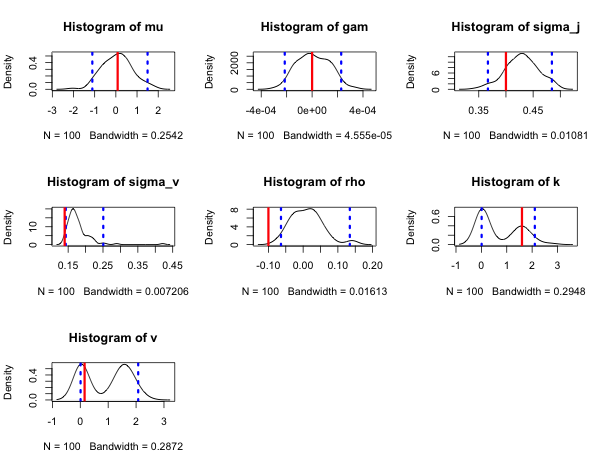
\includegraphics[scale=0.75]{density_plots}
\caption{95\% Credible Interval is denoted by the blue dotted line. True value of the parameter of the SVVG Model denoted by the red solid line.}
\end{figure}
\\
On average, the algorithm took 10-20 minutes for each sample path, resamples every 6-8 steps and runs for about 200 steps. From Table 1, 2 out of the 7 parameters do not lie within the 95\% credible interval. This could be due to the choice of $\Delta$ in the Euler Discretization which would affect the accuracy of the posterior parameter estimates. For this simulation, $\Delta$ was chosen to be $1/250$ to represent the daily close. One can choose a smaller $\Delta$ at the cost of higher complexity for the latent variables as one has to simulate data points between $(t,t+\Delta t)$. Note that from Table 1 and Figure 2, this SMC algorithm has been able to estimate $\mu$  quite accurately - a feature which we will use for our proposed Trading Strategy. From Figure 3, the acceptances are considered acceptable, since a Random-Walk Metropolis Kernel is used. However, there are some bouts of sensitivity of the rates during the middle of Iterations. But in general, the adaptive SMC Sampler has been able to prevent acceptance rates from going too low or too high.
\begin{table}
\centering
\begin{tabular}{|c c c c c|} 
 \hline
 Parameter & True & 0.025 & Median & 0.975 \\
 \hline
 $\mu$ & 0.085 & -1.1108 & 0.0595 &1.4978 \\
 $\gamma$ & 0.0 & -0.0002 & 0.0000 & 0.0002 \\
 $\sigma_{j}$ & 0.4 & 0.3668 & 0.4293 & 0.4845\\
 $\sigma_{v}$ & 0.14 & 0.1432 & 0.1693 &0.2508\\
 $\rho$ & -0.1 & -0.0638 & 0.0100 & 0.1344\\
 $\kappa$ & 1.6 & 0.0107 & 0.0479 & 2.1061\\
 $v$ & 0.155& 0.0109 & 1.2968 & 2.0762\\ 
 \hline
\end{tabular}
\caption{95\% Credible Interval and Median}
\label{table:1}
\end{table}
\begin{figure}
\centering
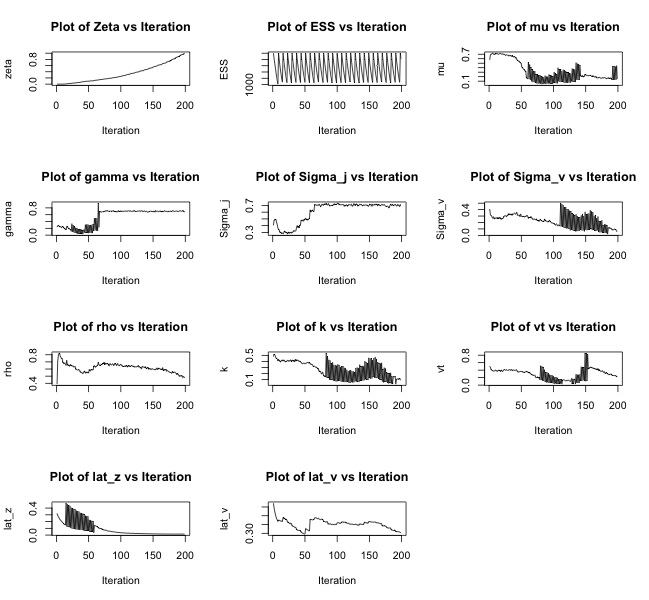
\includegraphics[scale=0.7]{acc_rates}
\caption{Plot of Acceptance Rates of Parameters vs Iteration}
\end{figure}


\subsection{The Trading Strategy}
For this section we will introduce a trading strategy using the result of the SMC Algorithm and see if it can outperform the traditional Buy and Hold (BnH) strategy. We will be using the daily data of S\&P500 from 3/1/2007 to 4/3/2016. Then given a user defined lookback period, $n$, we take a rolling window of $n$ Closes until 4/3/2016. Next, for each window, we perform the SMC algorithm to get us the posterior mean of $\mu$, which is the posterior expectation of the log returns of the instrument. After that, we generate buy/sell signals if $\mu>\mu_{thres}/\mu<-\mu_{thres}$. For the trading strategy, we take $n=30$, $\mu=0$. Also, we assume that we can buy/sell S\&P500 and that there are no transaction costs.\\
For comparison between strategies, the metric we will be using is called the CAR/MDD. It is simply the compounded annual return (CAR) divided by the max drawdown (MDD). Intuitively, a higher score means that our equity curve is smoother and therefore a better system.

\subsubsection{Naive Trading Strategy}

We model the trading strategy with zero transaction costs. The signal generated from the window of Closes is to be applied on the next day's Open. A positive/negative posterior mean would give a buy/sell signal for the next day. We will split the trading strategy into 2 separate portfolios that either buys or sells only. It is interesting to note that this naive strategy suffered a deep drawdown for the first 2.5 years, before it started to perform. Comparing between the buy and hold strategy and the Buy strategy, one can postulate that this is due to the initial weak performance of the Buy strategy.

\begin{figure}[H]
\centering
\begin{minipage}{0.5\textwidth}
  \centering
  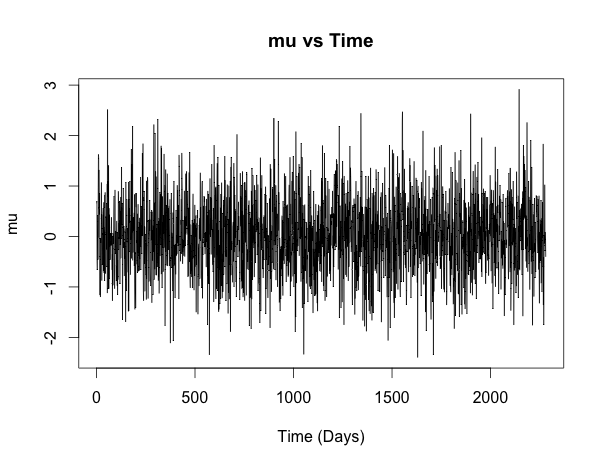
\includegraphics[width=1\textwidth]{ts1}
  \captionof{figure}{Plot of $\mu$ vs Time}
  \label{fig:test1}
\end{minipage}
\begin{minipage}{0.5\textwidth}
  \centering
  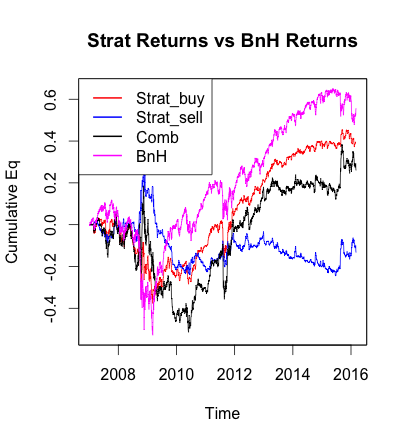
\includegraphics[scale=0.38]{ts2}
  \captionof{figure}{Plot of Equity vs TIme}
  \label{fig:test2}
\end{minipage}
\end{figure}

\begin{table}[H]
\centering
\begin{tabular}{|c|c|}
\hline
Strategy & CAR/MDD\\
\hline
Buy Only & 0.08463839\\     
Sell Only & -0.05490352\\
Combined & 0.01378244\\
BnH &  0.07773994\\
\hline
\end{tabular}
\end{table}

\subsubsection{The Improved Strategy}
We will now propose filters to filter out potential bad trades to try to increase profitability and improve the CAR/MDD. Using the first 500 observations as our training set (we select observations 1-500 for convenience), we will be using the following filters:
\begin{itemize}
\item Simple Moving Average (SMA) : To capture long term trends
\item Exponential Moving Average (EMA): To capture short term movements
%\item Direction of Previous Days: To follow momuntum
\end{itemize}
Our objective at the end of this is to create a portfolio of multiple trading strategies that hopes to produce superior returns, smoother equity curve and higher CAR/MDD ratio. In each of the trading strategies, we will optimise the input parameters (ie lookback period and $\mu_{thres}$) over the grid to get the highest CAR/MDD for the training set.\\
\bigskip
\textbf{\underline{Simple Moving Average Strategy}}\\
For the SMA trading strategy, we will use a simple moving average (with lookback period $n$) on the Open of SP500. The reason we calculate it on the Open is because the trading strategy can act upon the newest information, instead of using today's Close as a signal for tomorrow. Hence the trading rules are:
\begin{itemize}
\item Buy when Open is above the current SMA price \& $\mu>\mu_{thres}$
\item Sell when Open is below the current SMA price \& $\mu<-\mu_{thres}$
\end{itemize}
Next we optimise the Buy Strategy and Sell Strategy of the training set over the grids : $\mu_{thres} \in [0,1.0],n \in [3,60]$. The optimal parameters for the Buy and Sell strategies are $(0.8,60),(0.9,51)$ respectively. Next, we plot the whole equity curve (training + test sets) below. One may observe that the Sell strategy does not trade as often as one may expect - perhaps this is favourable because the SP500 has been increasing from 2009-2016 (and that Sell Strategies will tend to underperform under such conditions).
\begin{figure}[H]
\centering
\begin{minipage}{0.45\textwidth}
\centering
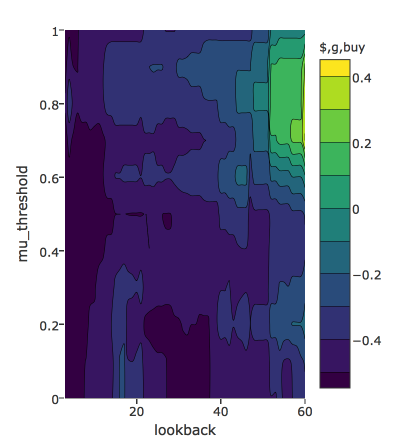
\includegraphics[scale=0.4]{contour1}
  \captionof{figure}{Contour for Buy Strategy (SMA)}
  \label{fig:c1}
\end{minipage}
\begin{minipage}{0.45\textwidth}
\centering
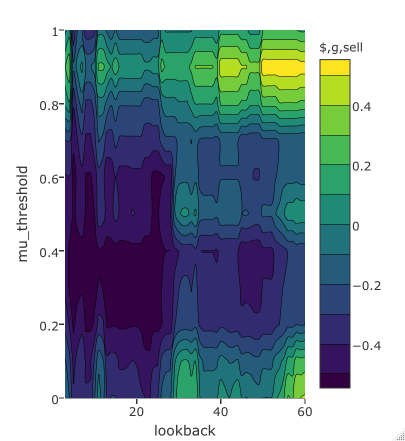
\includegraphics[scale=0.4]{contour2}
  \captionof{figure}{Contour for Sell Strategy (SMA)}
  \label{fig:c2}
\end{minipage}
\end{figure}

\begin{figure}[H]
\centering
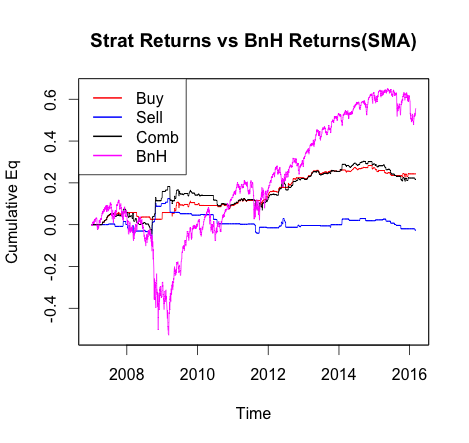
\includegraphics[scale=0.65]{combeq1}
  \captionof{figure}{Equity Curve for Optimised Buy/Sell Strategy (SMA)}
  \label{fig:c3}

\end{figure}

\begin{table}[h]
\centering
\begin{tabular}{|c|c|c|}
\hline
Strategy - SMA & CAR/MDD(Trg) & CAR/MDD(Test)\\
\hline
Buy Opt& 0.4022432 &0.34835462\\           
Sell Opt& 0.5756164 & -0.124869920\\
Combined Opt &0.5475945& 0.07000729\\
BnH &  -0.3938852 & 0.502743\\
\hline
\end{tabular}
  \captionof{table}{Statistics for Optimised Strategy (SMA)}
  \label{fig:c4}
\end{table}
\newpage
\justify
\textbf{\underline{Exponential Moving Average Strategy}}\\
Like the SMA trading strategy, we will use an exponential moving average (with lookback period $n$) on the Open of SP500. The trading rules are:
\begin{itemize}
\item Buy when Open is above the current EMA price \& $\mu>\mu_{thres}$
\item Sell when Open is below the current EMA price \& $\mu<-\mu_{thres}$
\end{itemize}
We optimise the Buy Strategy and Sell Strategy of the training set over the grids : $\mu_{thres} \in [0,1.0],n \in [3,60]$. The optimal parameters for the Buy and Sell strategies are $(0.4,3),(0.7,5)$ respectively. Next, we plot the whole equity curve (training + test sets) below. 
\begin{figure}[H]
\centering
\begin{minipage}{0.45\textwidth}
\centering
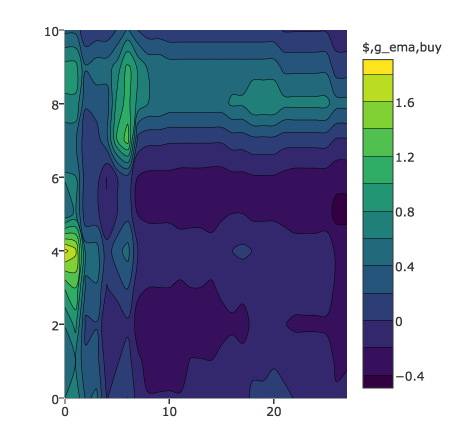
\includegraphics[scale=0.4]{contour3}
  \captionof{figure}{Contour for Buy Strategy(EMA)}
  \label{fig:c5}
\end{minipage}
\begin{minipage}{0.45\textwidth}
\centering
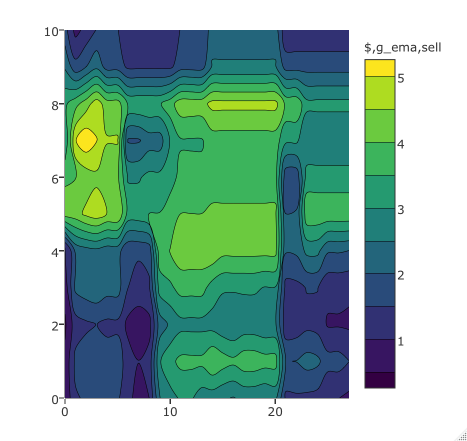
\includegraphics[scale=0.4]{contour4}
  \captionof{figure}{Contour for Sell Strategy(EMA)}
  \label{fig:c6}
\end{minipage}
\end{figure}

\begin{figure}[H]
\centering
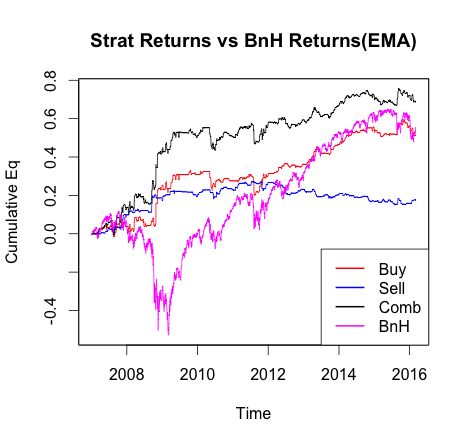
\includegraphics[scale=0.7]{combeq2}
  \captionof{figure}{Equity Curve for Optimised Buy/Sell Strategy (EMA)}
  \label{fig:c7}
\end{figure}

\begin{table}[H]
\centering
\begin{tabular}{|c|c|c|}
\hline
Strategy - EMA & CAR/MDD(Trg) & CAR/MDD(Test)\\ 
\hline
Buy Opt&1.852921& 0.3027411\\           
Sell Opt& 5.3704& -0.02609313\\
Combined Opt & 2.951226 &    0.3053557\\
BnH &  -0.3938852 & 0.5027435\\
\hline
\end{tabular}
\captionof{table}{Statistics for Optimised Strategy (EMA)}
\label{fig:c8}
\end{table}
\subsubsection{Combined Strategies}
Now that we have optmised the training sets of the 2 different strategies, we will now try to combine them into a single portfolio in hope of getting a smoother equity curve. We will optimise the strategies as follows:
\begin{itemize}
\item Step 1: Optimise weights $w_1,w_2,w_3,w_4$ (SMA Buy, SMA Sell, EMA Buy, EMA Sell respectively), based on the first 100 readings of the strategies.
\item Step 2: Walk the portfolio for the next $k$ days
\item Step 3: Re-optimise the weights using the past 100 days
\item Step 4: Iterate until end
\end{itemize}
We will set $k=20$ for this example. The plots and relevant statistics are shown below:
\begin{figure}[H]
\centering
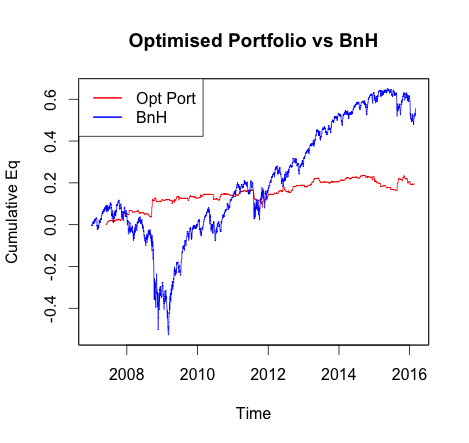
\includegraphics[scale=0.6]{last}
\end{figure}
\begin{table}[H]
\centering
\begin{tabular}{|c|c|}
\hline
Strategy & CAR/MDD\\
\hline
Opt. Portfolio & 0.2590368\\
BnH & 0.07773994\\
\hline
\end{tabular}
\end{table}
\newpage
\section{Conclusion}
In conclusion, we have introduced the L\'evy process and Sequential Monte Carlo and applied the simulation method on the SP500 to obtain the posterior estimates. The posterior estimates have been shown to be relatively accurate and one may tune the accuracy up by decreasing the delta in the Euler Discretisation. As for the implementation of the trading strategies, it is unfortunate that the strategies are unable to exceed the traditional buy and hold in terms of absolute returns even though it scores higher for the CAR/MDD. One reason could be that the strategies themselves (without incorporating information of the posterior estimates) are not known to be very profitable. In  all, this paper hopes to not only be a foundation for readers to get acquainted with the SMC and the Models that incorporates the L\'evy Process, but also to inspire further experimentation with the posterior estimates and trading strategies.

\section{Appendix}
$P(A_{n},..,A_{1}|B) = P(A_{n}|A_{n-1},..,B)P(A_{n-1}|A_{n-2},..,B)..P(A_{1}|B)$\\
Proof:
\begin{equation*}
\begin{split}
&P(A_{n}|A_{n-1},..,B)P(A_{n-1}|A_{n-2},..,B)..P(A_{1}|B)\\
 &= \frac{P(A_{n},A_{n-1},..,B)}{P(A_{n-1},A_{n-2},..,B)}\frac{P(A_{n-1},A_{n-2},..,B)}{P(A_{n-2},..,B)}...\frac{P(A_{1},B)}{P(B)}\\
 &= \frac{P(A_{n},..,A_{1},B)}{P(B)}\\
 &= P(A_{n},..,A_{1}|B)\\
 \end{split}
\end{equation*}\\
\bigskip
If $p_{t} \approx p_{t+1}$, then $\widetilde{w}_{t+1}^{i}(\theta_{t},\theta_{t+1}) = \frac{\gamma_{t+1}(\theta_{t})}{\gamma_{t}(\theta_{t})}$ \\
Proof:\\
Using equations \ref{eq:6} and \ref{eq:7},\\
\begin{equation*}
\begin{split}
\widetilde{w}_{t+1}^{i}(\theta_{t},\theta_{t+1}) &= \frac{\gamma_{t+1}(\theta_{t+1})L_{t}(\theta_{t+1},\theta_{t})}{\gamma_{t}(\theta_{t})K_{t+1}(\theta_{t},\theta_{t+1})}\\
&= \frac{\gamma_{t+1}(\theta_{t+1})}{\gamma_{t}(\theta_{t})K_{t+1}(\theta_{t},\theta_{t+1})}\cdot \frac{p_{t+1}(\theta_{t})K_{t+1}(\theta_{t},\theta_{t+1})}{p_{t+1}(\theta_{t+1})}\\
&= \frac{\gamma_{t+1}(\theta_{t+1})}{\gamma_{t}(\theta_{t})}\cdot \frac{p_{t+1}(\theta_{t})}{p_{t+1}(\theta_{t+1})}\\
&= \frac{\gamma_{t+1}(\theta_{t+1})}{\gamma_{t}(\theta_{t})}\cdot \frac{\frac{\gamma_{t+1}(\theta_{t})}{Z_{t+1}}}{\frac{\gamma_{t+1}(\theta_{t+1})}{Z_{t+1}}}\\
&= \frac{\gamma_{t+1}(\theta_{t})}{\gamma_{t}(\theta_{t})}
\end{split}
\end{equation*}
where we have used the fact that $p_{t} = \frac{\gamma_{t+1}(\theta_{t})}{Z_{t+1}}$,$Z_{t+1}:=$ the normalisation constant.\\

\addcontentsline{toc}{section}{References}
\bibliographystyle{IEEEtran}
\bibliography{/Users/Joel/Desktop/smc/report/smc.bib}
\end{document}


